\documentclass[10pt]{beamer}
\usepackage{amsmath}
% Bold Math
\usepackage{bm}
\usepackage[font=footnotesize]{caption}
% Dashed horizontal lines
\usepackage{arydshln}
% For spacing between underbrace and text
% \addstackgap[6pt]
\usepackage{IEEEtrantools,stackengine}

\usetheme{Boadilla}

\title{Master Thesis -- 3 Week Presentation}
\subtitle{The Langevin Approach to Discretise the Collision Operator}
\author{Tobia Claglüna}
\institute{AMAS - PSI}
\date{\today}


\begin{document}
 \begin{frame}
     \titlepage
 \end{frame}

 \begin{frame}
     \frametitle{Outline}
     \tableofcontents
 \end{frame}

 \section{Governing Equations}

 \begin{frame}
\linespread{2.5}\selectfont
     \frametitle{Vlasov Equation}
     Describes the evolution of phase space including long-range interactions
     \begin{equation}
         \frac{\partial f(\bm r,\bm v)}{\partial t} + \bm{v} \cdot \frac{\partial f}{\partial \bm r} + \frac{\bm{F}}{m} \cdot \frac{\partial f}{\partial \bm v} = \left(\frac{\partial f}{\partial t}\right)_{\text{coll}}
     \end{equation}

     Use Fokker-Planck (FP) equation to define the collision dependent term.


 \end{frame}

 \begin{frame}
     \frametitle{From a Markov Process to Fokker-Planck}

	 \begin{itemize}
	 \setlength{\itemsep}{10mm}
		 \item Markovian assumption holds if $t_c \ll \Delta t$ \\
		 \item By Taylor expansion of density change we arrive at

			 \begin{equation}
				 \left( \frac{\partial f(\bm v)}{\partial t}\right)_{\text{coll}} = -\frac{\partial}{\partial v} \cdot (f \underbrace{\addstackgap[6pt]{\langle \Delta\mathbf{v} \rangle}}_{\bm{F_d}}) + \frac{1}{2} \frac{\partial^2}{\partial \mathbf v \partial \mathbf v} : (f \underbrace{\addstackgap[6pt]{\langle \Delta \mathbf{v} \Delta \mathbf{v^T} \rangle}}_{\bm{D}})
			 \end{equation}
			 \\
			 Doesn't require the system to be in thermal equilibrium
			 %\newline

		 \item Compute the Dynamical Friction $\bm{F_d}$ and Diffusion coefficients $\bm D$ by describing the scattering mechanism.
	 \end{itemize}

 \end{frame}

\section{Collisions - Rosenbluth Potentials}

 \begin{frame}
     \frametitle{Elastic collisions}
     Simplifying assumptions:
     \begin{itemize}
	 \setlength{\itemsep}{3mm}
         \item Single species medium
         \item Consider collisions as binary events (in particle frame)
         \item Ignore small angle deflections by defining a minimum scattering angle $\theta_{\text{min}} = \theta(\lambda_D)$ (Debye Shielding)
     \end{itemize}

     \begin{equation}
         \bm{F_d} = \langle \Delta\mathbf{v} \rangle = \int f(\bm v) \int u \Delta \bm v \sigma(u, \Omega) d\Omega d\bm v 
     \end{equation}

	 \begin{columns}
		 \column{0.4\textwidth}
		 	Use Rutherford cross-section for Coulomb interactions: 
			\newline \newline
				$\sigma(u, \Omega) = \left(\frac{q^2}{8 \pi \epsilon_0 m u^2} \right)^2 \frac{1}{sin^4(\theta/2)}$
		 \column{0.5\textwidth}
		 \begin{figure}
			 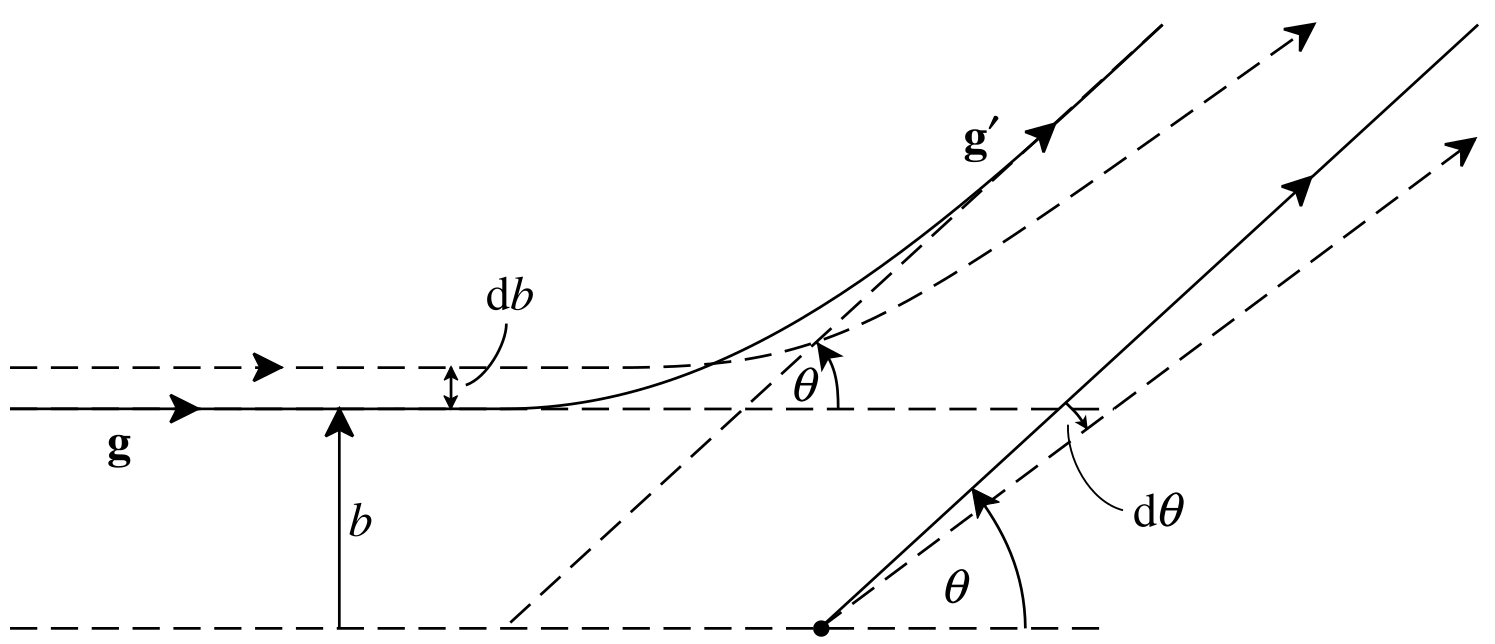
\includegraphics[scale=0.1]{figures/scattering.png}
			 \caption{Binary Scattering \cite{boyd_sanderson_2003}}
			 \label{fig:scattering}
		 \end{figure}
	 \end{columns}

     %\begin{equation}
         %\langle \Delta\mathbf{v} \Delta\mathbf{v^T} \rangle = \int f(\bm r, \bm v) \int u \Delta \bm v \sigma(u, \Omega) d\Omega d\bm v 
     %\end{equation}

 \end{frame}


 \begin{frame}
 \frametitle{Rosenbluth Potentials \cite{rosenbluth}}

	 \begin{columns}[t] 
		 \begin{column}{0.5\textwidth}
 Potentials on velocity space only \cite{PlasmaKineticTheory}:
 \begin{align}
	 \Gamma   &= \frac{q^4 \ln(\Lambda)}{4 \pi \epsilon_0^2 m^2} \\[9pt]
	 H(\bm v) &=  2 \int d^3 v^\prime \frac{f(\bm{v^\prime})}{|\bm v - \bm{v^\prime}|} \\[9pt]
	 G(\bm v) &=  \int d^3 v^\prime f(\bm{v^\prime}) |\bm v - \bm{v^\prime}| \\[9pt]
	 \langle \Delta\mathbf{v} \rangle &=  \Gamma \frac{\partial H}{\partial \bm v} = \bm{F_d} \\[9pt]
	 \langle \Delta\mathbf{v}\Delta\mathbf{v}^T \rangle &=  \Gamma \frac{\partial^2 G}{\partial \bm v \partial \bm v} = \bm D
 \end{align}	
 \end{column}
 \hspace{-8pt}
 \vrule{}
 \hspace{+7pt}
		 \begin{column}{0.4\textwidth}
 Resulting Elliptic Identities: \\[6pt]
 \begin{align}
	 \nabla_{\bm{v}}^2 \nabla_{\bm{v}}^2 G(\bm v) &=  -8 \pi f(\bm v) \\[21pt]
	 \nabla_{\bm{v}}^2 G(\bm v) &= H(\bm v)
 \end{align}	
 \end{column}
\end{columns}

 \end{frame}

\begin{frame}
\frametitle{Resulting Scheme \cite{stoel}}

\begin{equation}
\frac{\partial f}{\partial t} + \bm{v} \cdot \frac{\partial f}{\partial \bm r} + \frac{\bm{F}}{m} \cdot \frac{\partial f}{\partial \bm v} = -\frac{\partial}{\partial v} \cdot (f \bm{F_d}) + \frac{1}{2} \frac{\partial^2}{\partial \mathbf v \partial \mathbf v} : (f \bm D)
\end{equation} \newline

Langevin type formulation of the Vlasov equation with the FP collisional term \cite{Risken1984FokkerPlanckE}:

\begin{equation}
\left\{
 \begin{align}
	 \quad \frac{d \bm r}{dt} &= \bm v \\
	 \frac{d \bm v}{dt}  &=  \frac{\bm F}{m} + \bm F_d + \bm Q \cdot d\bm W_t \\
	 \bm D &= \bm Q \bm Q^T
 \end{align}	
\right.
\end{equation}

Also works for the non-electrostatic case!


\end{frame}

\section{Disorder Induced Heating}

\begin{frame}
\frametitle{Disorder Induced Heating}

\begin{itemize}
	 \setlength{\itemsep}{3mm}
	\item Cold coasting electron beam
	\item Collisions cause beam temparature to rise (undesired)
	\begin{itemize}
		\setlength{\itemsep}{2mm}
		\item Beam widens
		\item Emittance increases
	\end{itemize}
\end{itemize}

\begin{figure}
	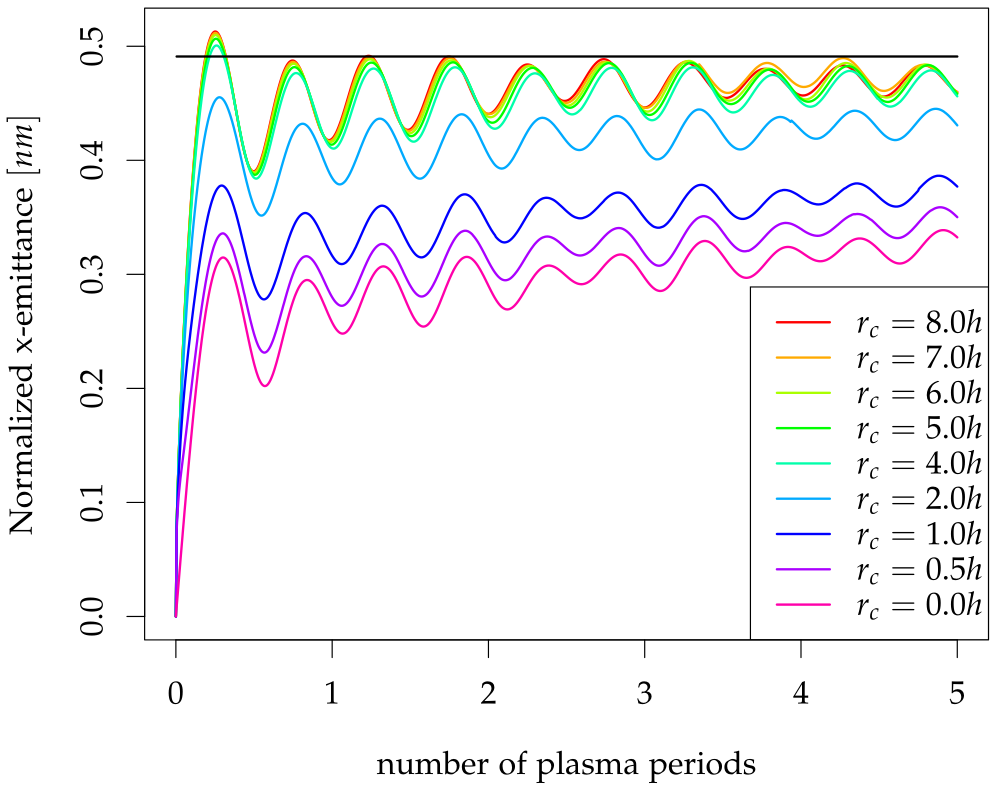
\includegraphics[scale=0.17]{figures/dih_ulmer.png}
	\caption{DIH resolved with P\textsuperscript{3}M \cite{p3m_ulmer}}
	\label{fig:DIH_p3m}
\end{figure}

\end{frame}

\section{Timeline}

\begin{frame}
\frametitle{Timeline I}
\begin{table}[]
\def\arraystretch{1.5}
\begin{tabular}{p{0.08\linewidth} | p{0.85\linewidth}}
Date & Target Goals \\
\hline \hline
30/01 & Assist Severin and ensure correctness of current implementation \\
20/02 & Find Order of convergence / accuracy and compare whether really much better than P3M (even though it might still run only on single core) \\
20/02 & Ensure Performance Portability (MPI, OpenMP and GPU) \\
06/03 & Benchmarking of accuracy, runtime and scalability \\
27/03 & Start improving most pressing bottlenecks \\
\textcolor{gray}{03/04} & \textcolor{gray}{Easter Holidays} \\
01/05 & Research on better integrators / explore Multi-Level Monte-Carlo approach \\
\end{tabular}
\caption{Timeline with approximate milestones}
\end{table}

\end{frame}

\begin{frame}
\frametitle{Timeline II}

\begin{table}[]
\def\arraystretch{1.5}
\begin{tabular}{p{0.08\linewidth} | p{0.85\linewidth}}
Date & Target Goals \\
\hline \hline
08/05 & Implement algorithmic improvements and compare accuracy / performance to previous implementation \\
29/05 & (Potential Implementation into OPAL via IPPL-1 implementation) \\
12/06 & Start writing and code clean-up \\
03/07 & Submission \\
\end{tabular}
\caption{Timeline with approximate milestones}
\end{table}

\end{frame}

 \begin{frame}[allowframebreaks]
     \frametitle{References}
     \bibliographystyle{apalike}
     \bibliography{refs.bib}
 \end{frame}
 

\end{document}

